\pagenumbering{gobble}
	\underline{\textbf{Architectural design} }
	\begin{legal}
    		\item \textit{\textbf{Overview: high-level components and their interaction}}\\\\
The figure below represents an high level overview of the system. Further details
on the system components and their interaction will be further explained in the next sections.\\
		\begin{figure}[H]
		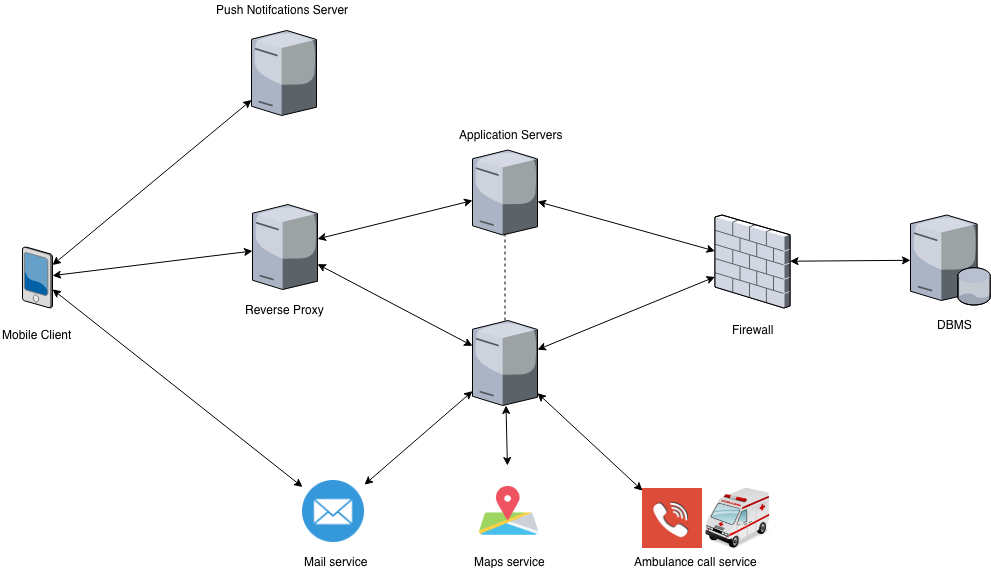
\includegraphics[width=\linewidth]{../images/OverviewDiagram.png}
		\end{figure}
		\item \textit{\textbf{Component view}}\\\\
		%s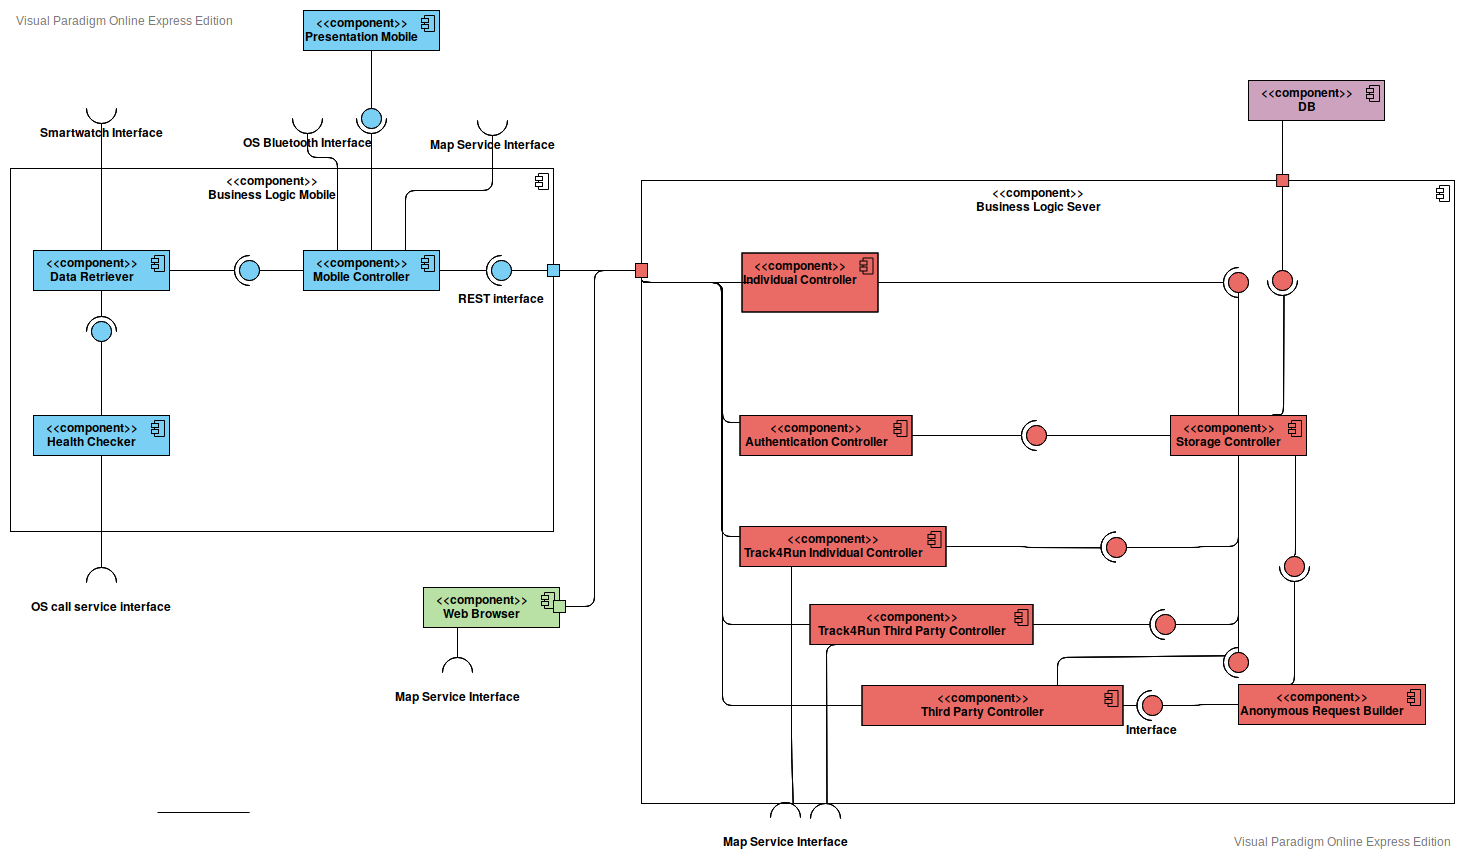
\includegraphics[width=\linewidth]{../images/ComponentDiagram.png}
		\item \textit{\textbf{Deployment view}}\\\\
		The figure below shows the deployment diagram of the whole system. Its main goal is to describe the distribution of components capturing the topology of the
system's hardware.\\
		\begin{figure}[H]
		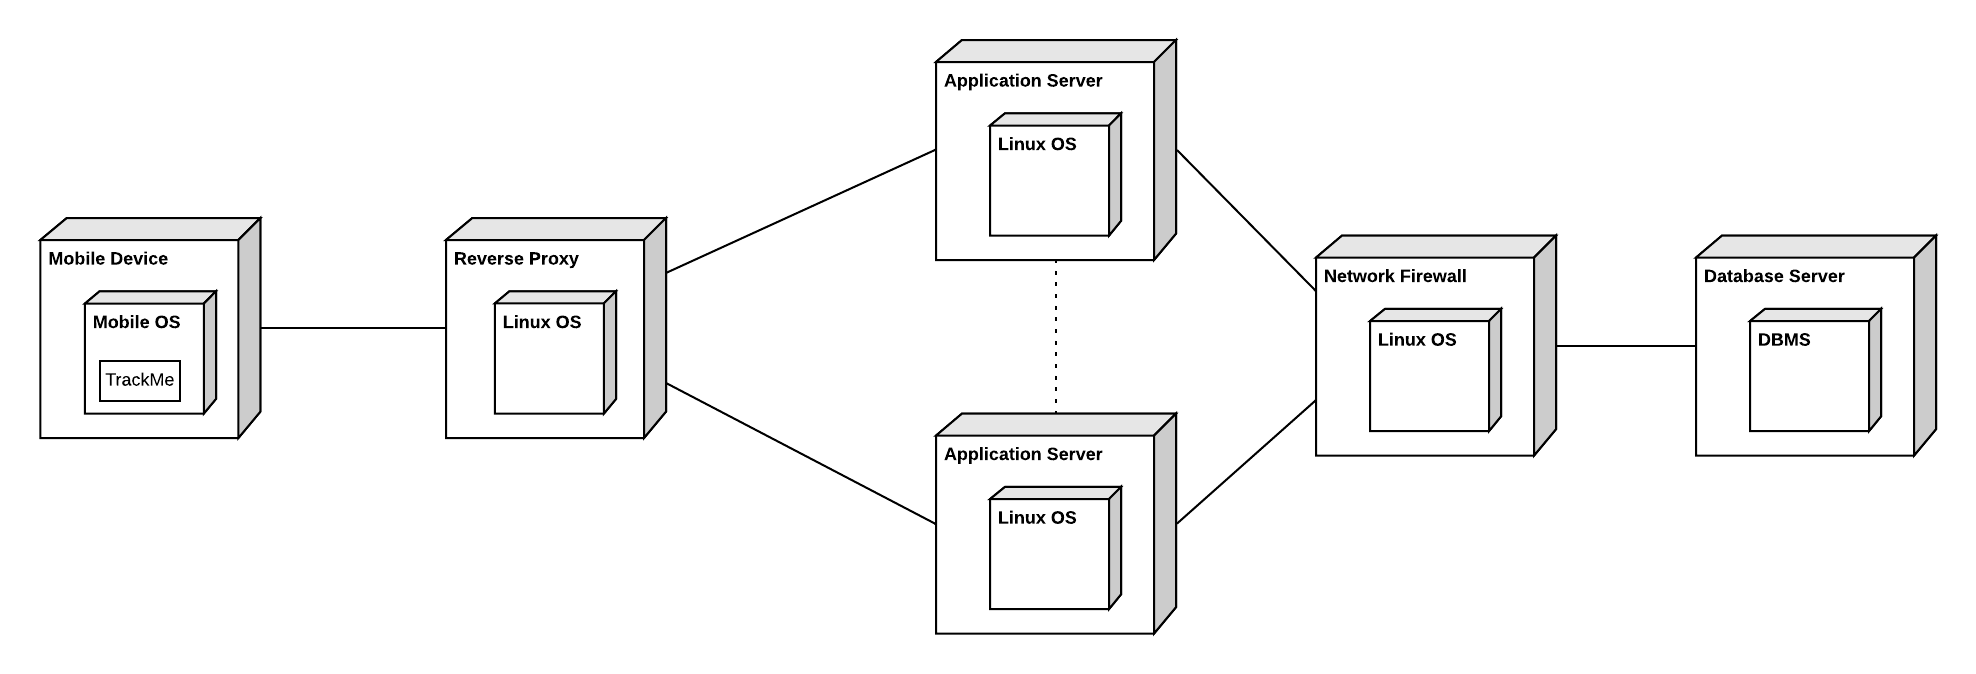
\includegraphics[width=\linewidth]{../images/DeploymentDiagram.png}\\
		\end{figure}
		As previously stated in the section 1, the system is structured in a multi-tier architecture. The specific role of each node is clarified here:\\\\
		\textbf{Clients}\\
The first tier is composed by the mobile clients machines. The client will be able to access TrackMe functionalities through the dedicated native application.\\\\
		\textbf{Reverse Proxy}\\
We chose to deploy a reverse proxy on a Linux machine with Nginx server installed on it, in order to safely increase parallelism of requests and scalability
of our application. This architecture leads to several advantages:
		\begin{itemize}
			\item Load balancing, distributing requests among different servers
			\item Optimising content by compressing it in order to speed up loading times
			\item Event-driven architecture, increasing parallelism by not locking the CPU
			\item Very conservative memory-wise\\
		\end{itemize}
		\textbf{Application Servers}\\
This is the middleware level of the architecture: all the business logic of
the system is contained in these servers.\\\\
		\textbf{Network Firewall}\\
The access to the Database is mediated by a network firewall in order to
avoid unauthorised access to the data and the credentials of the user.\\\\
		\textbf{Database Server}\\
This is the last layer of the architecture: all the data are stored in a Database Server accessed through a relational DBMS. \\\\
		\item \textit{\textbf{Runtime view}}\\
			\begin{legal}
				\item \textbf{Sign up Runtime View}\\
				\item \textbf{Login Runtime View}\\
				\item \textbf{Join a run Runtime View}\\
				\item \textbf{Organise a run Runtime View}\\
				\item \textbf{Individual request Runtime View}\\
				\item \textbf{Group request Runtime View}\\
			\end {legal}
		\item \textit{\textbf{Component interfaces}}\\\\
		\item \textit{\textbf{Selected architectural styles and patterns}}\\\\
  	\end{legal}
